\chapter{Evaluation and Testing}

This chapter critically evaluates the final artefact and its development process against the previously defined constraints, functions, and methodology outlined within chapters: one, three, four, and the Project Initiation Document displayed within Appendix A.

\section{Aims and Objectives Evaluation}

\begin{figure}[H]
    \centering
    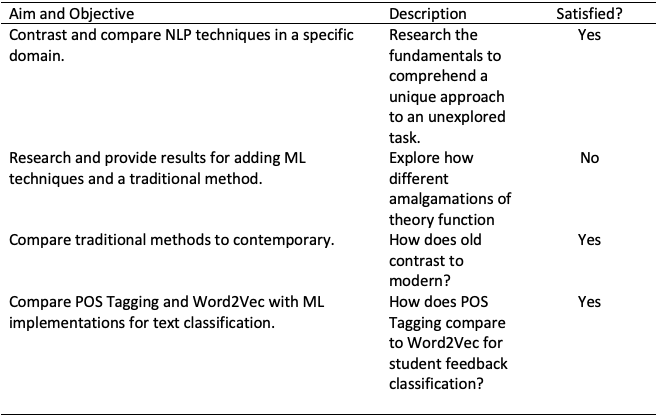
\includegraphics[width=\textwidth]{figures/chapter-7/AimsAndObjectives.png}
    \caption[Evaluation of Aims and Objectives]{Evaluation of Aims and Objectives.
    \label{fig:aimsandobjectives}}
\end{figure}

\section{Methodology}

The selected methodological approach was best suited because of the project's basis, at the lowest level of abstraction, this project relates to data-mining and analytics, therefore, the CRISP-DM model was an accurate SDLC to apply throughout the development phase. As shown in \autoref{chapter:methodologyprojectplanning}, there are two separate SDLC, one relates to the overall project (CRISP-DM) and the other is tailored towards the machine learning development side, this secondary model was very insightful when issues arose and gave a clear path on how to take the necessary steps towards solving said issue. \autoref{fig:MLDC} is an agile focused SDLC with aspects of the iterative approach, using an agile approach felt most appropriate given machine learning projects can change their requirements frequently, agile methods also work well with KANBAN boards which this project makes use off. Therefore, the overall methodology seems most appropriate for this project in its entirety.

\subsection{Project Plan}

The initial project plan touched upon within the Project Initiation Document was satisfactory as the developer did not know where or how the project would veer from any original planning concepts, therefore, the initial project plan was sufficient in which it gave a baseline on how to proceed with each stage of execution. As stated within the PID, time management issues were very likely to appear in which they did, severely hindering the progress of this project to which did result in failure regarding some project requirements.

\section{Requirement Evaluation}

\subsection{Functional Evaluation}

\begin{figure}[H]
    \centering
    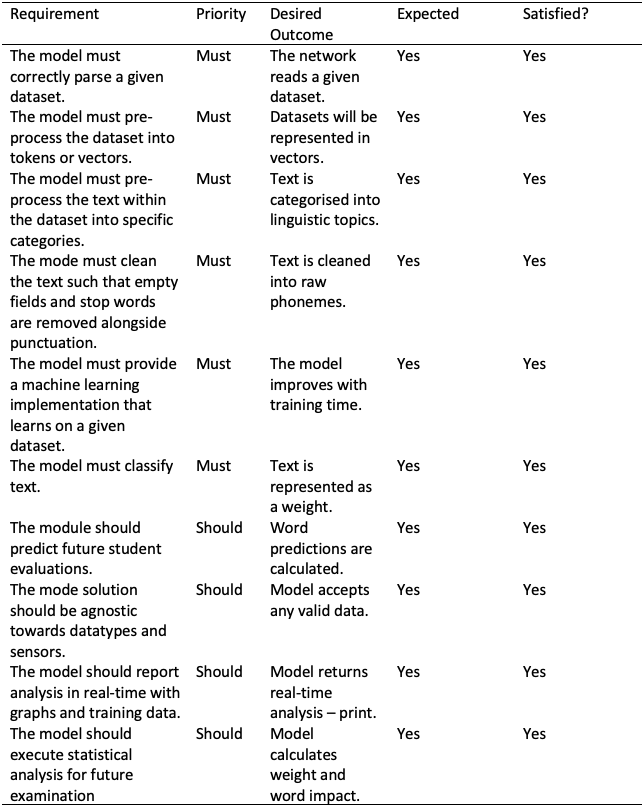
\includegraphics[width=\textwidth]{figures/chapter-7/FunctionalEval.png}
    \caption[Evaluation of Functional Requirements]{Evaluation of Functional Requirements.
    \label{fig:FunctionalEval}}
\end{figure}

\subsection{Non-Functional Evaluation}

\begin{figure}[H]
    \centering
    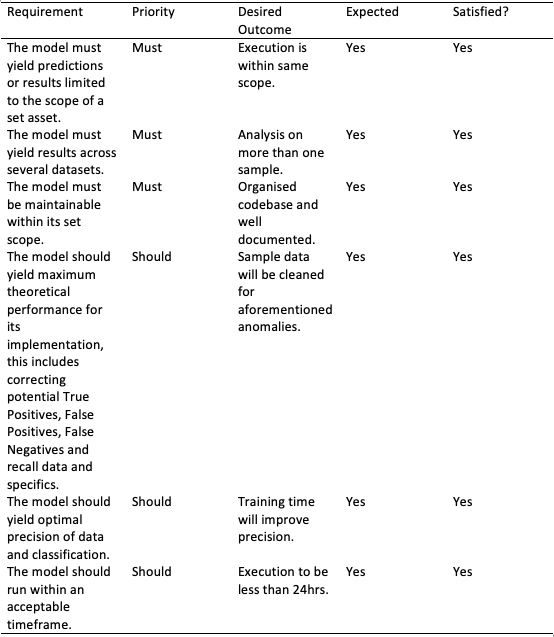
\includegraphics[width=\textwidth]{figures/chapter-7/NonFunctionalEval.png}
    \caption[Evaluation of Non-Functional Requirements]{Evaluation of Non-Functional Requirements.
    \label{fig:NonFunctionalEval}}
\end{figure}

\newpage

\section{Artefact Evaluation}

This project saw major setbacks, to which minimised the project potential for comparing different natural language processing techniques against the respected theory, as development was carried out, it became apparent that not all of the intended functionality would be able to be implemented into the golden-master branch (the final deployment of the model), however, the artefact still shows potential for performance updates and increases to training accuracy whereby the embedding matrix can have a higher weight towards word units for classification within the contemporary implementation. Even though both models were not synthesized, the final artefact can be seen as a success is its own right for textual classification and student feedback prediction.

The implemented model displays deep natural language processing theory and understanding to which would not be of use unless a successful deployment could occur, this artefact also successfully translated a theoretical mathematical approach into a programming object, given the use of several helper libraries.

Overall, this project did not finalise into what was expected at project start, or delivery what was expected (two different model variants); however, the model that was implement was successful and did meet a majority of the functional and non-functional requirements.

\subsection{Testing}

\begin{figure}[H]
    \centering
    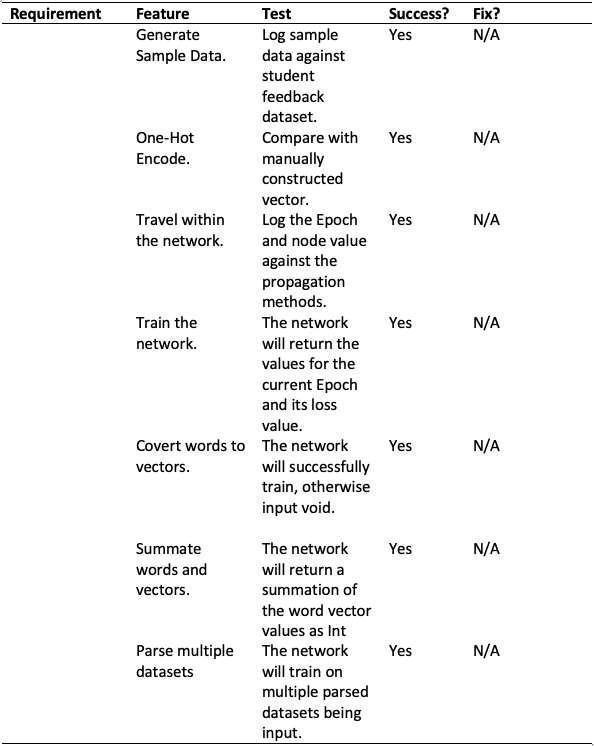
\includegraphics[width=\textwidth]{figures/chapter-7/Testing.png}
    \caption[Evaluation of Artefact Testing]{Evaluation of Artefact Testing.
    \label{fig:Testing}}
\end{figure}